\chapter{Conception}
Passant du cadre théorique à l'application pratique, cette section décrit la conception et le flux opérationnel de notre pipeline bioinformatique
\section{Flux opérationnel}
Voici un diagramme reprenant les différents points de la conception de notre travail.
\begin{center}
    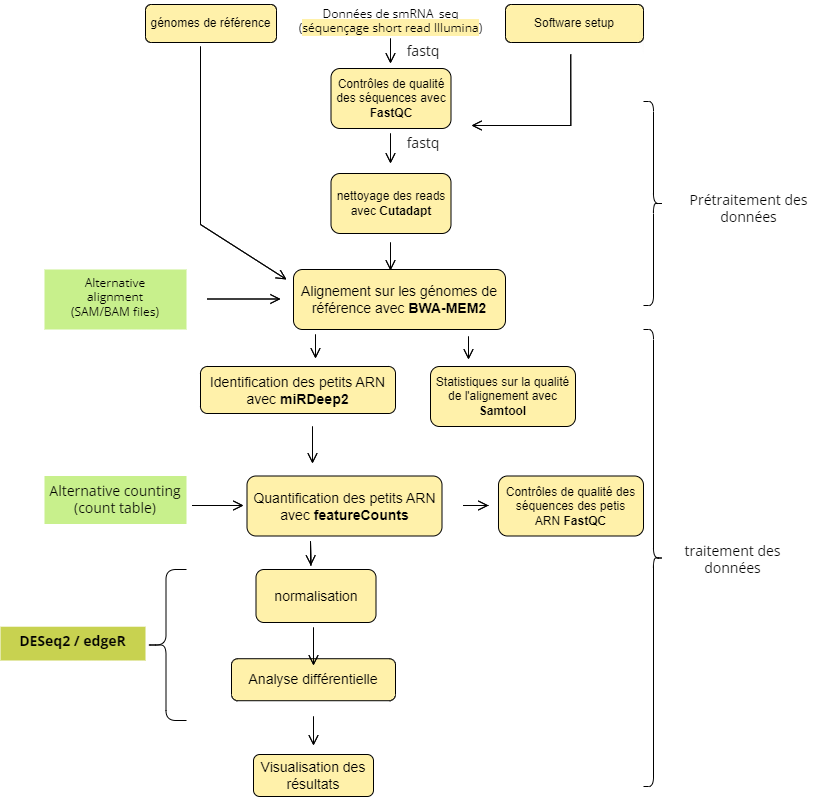
\includegraphics[scale=0.5]{img/PIPLINE_RNA.png}\\[1cm]
\end{center}

\section{Contrôle de qualité}
Les séquences que le client nous a fournis stockées dans des fichiers sont soumises à deux nombreuses erreurs potentielles. Avant d’arriver dans les fichiers, les séquences ont été extraites de matériel vivant, isolées, lavées, préparées, amplifiés, séquencées… la liste est longue. Afin de vérifier qu’au cours de ces étapes précises, le matériel biologique a correctement été transcrit dans les Fastq un contrôle qualité de ces derniers est nécessaire. 

Le contrôle qualité est une étape très classique appliqué sur des séquences de nucléotides. On en extraira de nombreuses métriques qui pourront nous indiquer d’une part si le séquençage s’est bien déroulé mais aussi nous donner des indications de l’anatomie générale des reads que nous avons obtenus. \\

\noindent Parmi les mesures que nous obtiendrons grâce à notre contrôle qualité, nous allons garder un œil sur plusieurs d’entre eux :
\begin{itemize}
    \item  La taille moyenne des reads devrait se rapprocher des tailles des miARN attendus. 
    \item La qualité de lecture des bases devrait être forte car nous somme en short reads. 
    \item De nombreuses séquences d’adaptateurs devrait être présentes dans nos échantillons car ils ont été utilisés pour la préparation des miARN. Leur présence devrait se traduire par un grand nombre de séquences dupliquées. 
\end{itemize}


\section{Nettoyage des reads (trimming)}
Après avoir effectué un contrôle qualité des séquences, il est apparu que plusieurs traitements étaient nécessaires sur les fichiers bruts avant de pouvoir les exploiter. Le trimming représente une étape cruciale car il permet d'éliminer les séquences superflues en vue de nos analyses futures. De plus, certaines parties des reads peuvent avoir été utilisées pour leur indexation, rendant ainsi indispensable leur suppression afin de restaurer un contexte biologique cohérent.


\subsection*{Trimming classique}
Lors de l'utilisation standard d'un outil de filtrage des séquences, nous débutons par la discrimination des lectures de bases de mauvaise qualité. En effet, nos données de séquençage, stockées dans des fichiers FastQ, associent chaque base à un score de qualité Phred. Ce score nous renseigne sur la probabilité que la lecture de la base actuelle soit incorrecte. Ainsi, pour garantir la fiabilité des données, il est nécessaire d'éliminer toutes les bases présentant une forte probabilité d'erreur \cite{phread}.\\


Les séquençages Illumina présentent une perte de qualité croissante selon la longueur du fragment, attribuable aux méthodes de production. Ainsi, les bases de faible qualité se retrouvent souvent du côté 3’ du brin d'ARN. Pendant le trimming, nous éliminerons les bases en 3’ une par une jusqu'à ce qu'il ne reste plus de bases de faible qualité. Ce processus réduit légèrement la taille moyenne des fragments, mais dans notre cas de séquençage de miARN, ces derniers sont si courts que la qualité n'a pratiquement pas le temps de diminuer.\\

Ensuite, le séquençage Illumina nécessite l'utilisation d'adaptateurs pour fixer les ARN sur la flowcell avant amplification. Bien que ces séquences soient nécessaires, elles doivent être retirées des lectures avant leur étude \cite{illumina}. 

\begin{SCfigure}[1][h]
    \centering
    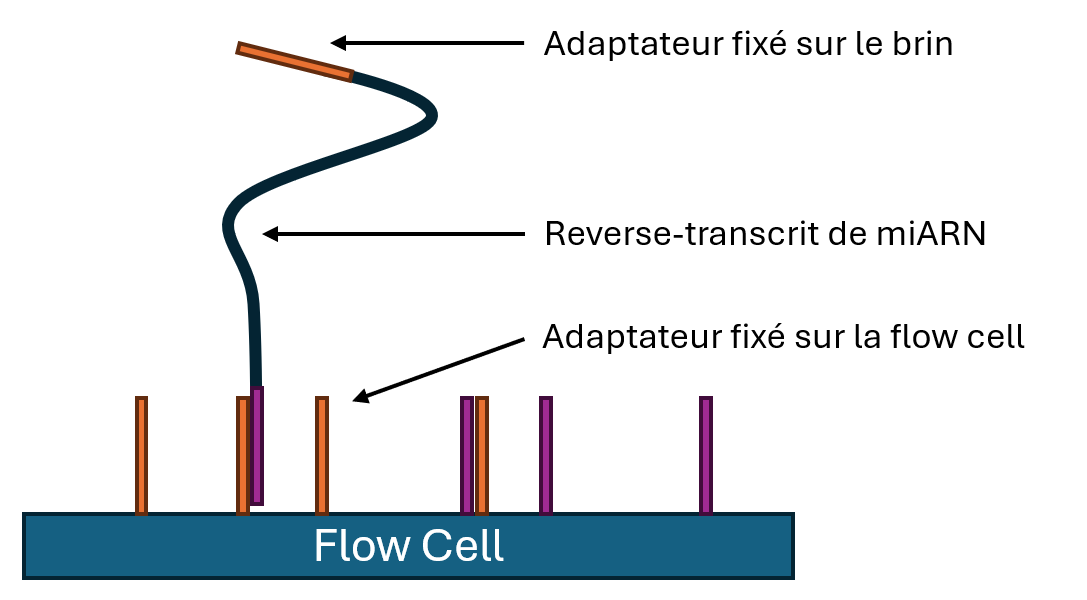
\includegraphics[width=0.5\textwidth]{img/flowcell.PNG}
    \caption{Schéma d'une flowcell fixant un brin d'ADN reverse transcrit à partir d'une séquence de miARN}
    \label{fig:flowcell}
\end{SCfigure}

\subsection*{Trimming additionnel}
\noindent Au-delà des adaptateurs spécifiques à Illumina, nos données contiennent de nombreuses autres séquences qui doivent être supprimées. Voici une liste exhaustive des adaptateurs supplémentaires :

\begin{itemize}
    \item Les \textbf{adaptateurs miRNA} : présents en 5’ et 3’, ils permettent d'améliorer considérablement les séquençages short reads des petits ARN.
    \item Les \textbf{séquences I5 et I7} : elles permettent de différencier plusieurs échantillons dans une même expérience, et sont uniques pour chaque condition expérimentale, étant présentes en 5’ et 3’.
    \item Enfin, avant l'adaptateur Illumina, une \textbf{UDI (Unique Dual Index)} est présente en 3’, permettant le multiplexage entre différentes expériences. Cela permet d'optimiser les ressources en introduisant une grande quantité de matériel génétique dans le séquenceur.
\end{itemize}

\begin{figure}[ht]
    \centering
    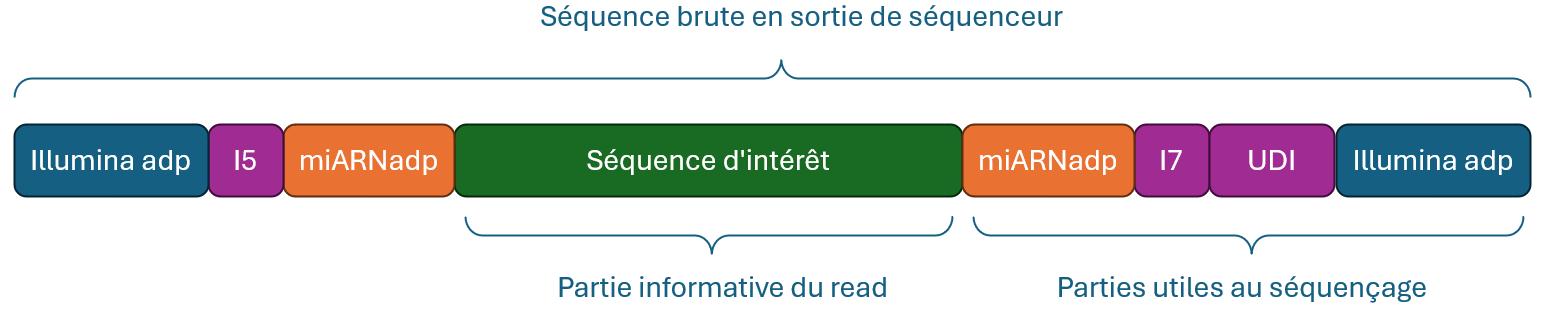
\includegraphics[width=1\textwidth]{img/sequence.PNG}
    \caption{Diagramme illustrant la composition des séquences brutes.}
    \label{fig:sequence}
\end{figure}

Notre code est confronté à un défi majeur : les séquences I7 et I5, qui permettent de différencier les échantillons, sont uniques pour chaque condition expérimentale. Par conséquent, nous devons les retirer de manière dynamique. Pour gérer cette problématique, nous avons créé un fichier CSV (valeurs séparées par des virgules) qui servira de base de données pour sélectionner les différentes séquences à retirer. Les séquences I7/5 concernées seront intégrées à l'outil aux côtés des adaptateurs Illumina, des miARN et de l'UDI.\\

\section{Alignement des séquences}
Une fois nos séquences nettoyées, nous allons les aligner sur leurs génomes de référence afin de caractériser leurs emplacements. Cette étape est cruciale car elle permettra d’avoir une visualisation plus globale de nos données. 

Deux complications nous font faces pour cet alignement. Tout d’abord la nature même de nos séquences rend difficile leur localisation, les reads de miARN font environ 22 nucléotides de long ce qui laisse place à des erreurs d’alignement notamment sur les zones conservées de ces derniers.

D’autre part, nous avons des échantillons qui sont mesurées dans des situations de coculture. Quand la coculture est effectuée entre différente souches, il faudra être capable d’aligner sur plusieurs génomes de références. 

\section{Identification des miARN}
Grace a l’alignement, des séquences, une identification des miARN sera possible. Cette dernière marquera le dernier traitement sur les données que nous effectuerons. Elle permettra d’apprécier les types de miARN produits et leurs quantités dans chaque zone du génome. Nous regarderons notamment la quantité d’ARN ribosomique ainsi que la position des reads au sein des régions non codantes. 

Cette identification nous permettra d’observer si la variabilité au sein de cette population de miARN est forte ou s’ils sont dominés par des groupes bien définis. Mais surtout nous pourrons comparer quantitativement les scénarios de coculture et de monoculture pour essayer d’identifier les potentiels ARN qui sont plus produit dans les cas ou deux champignons sont confrontés. 

Après normalisation, si le ratio de différence d’expression d'un ANR entre des conditions expérimentales est élevé, ces derniers seront des cibles de choix pour des études plus poussé sur leurs fonctions propres. 

\section{Le Pipeline}
Le pipeline sera découpé en plusieurs scripts qui jongleront entre eux avec les données. Cette approche permet une modularité accrue, facilite la gestion et la réutilisation du code. Si, dans le futur, le client souhaite adapter le pipeline à deux nouveaux besoin, il lui suffira de modifier un seul script. 
Les résultats d'une étape alimentent la suivante, ainsi, tant que les formats de fichiers sont respectés le programme pourra fonctionner. Cela permet aussi d'utiliser plusieurs langages et prendre le mieux adapté pour chaque étape du pipeline.

